\documentclass[quiz]{mcs}

\renewcommand{\exampreamble}{   % !! renew \exampreamble
\iffalse
  \textbf{Circle the name of your TA}:
  \begin{center}
  \renewcommand{\arraystretch}{2.5}
  \begin{tabular}{l}
     \courseassistants
  \end{tabular}
  \end{center}\fi

  \begin{itemize}

  \item This exam is \textbf{closed book} except for a two page, 2-sided
    crib sheet.  Total time is 3 hours.

  \item Write your solutions in the space provided with your name on every
    page.  If you need more space, write on the back of the sheet
    containing the problem.  Please keep your entire answer to a problem
    on that problem's page.

  \item
   GOOD LUCK!
  \end{itemize}}

% omitted topics: bijection, uncountable; constraint scheduling; set
% properties; quantifiers; recurrences; graph isomorphism, connectivity; 
% RSA ??

\begin{document}
\final

%%%%%%%%%%%%%%%%%%%%%%%%%%%%%%%%%%%%%%%%%%%%%%%%%%%%%%%%%%%%%%%%%%%%%
% Problems start here
%%%%%%%%%%%%%%%%%%%%%%%%%%%%%%%%%%%%%%%%%%%%%%%%%%%%%%%%%%%%%%%%%%%%%

%\examspace
%  \pinput[points = 5, title= \textbf{Logic and Relations}]{FP_logic_relations}

%\examspace
%  \pinput[points = 5, title = \textbf{Logic and Graphs and Probability, oh my!}]{FP_graph_logic_probability}
 
\examspace
  \pinput[points = 5, title = \textbf{Asymptotic Bounds and Partial Orders}]{FP_asymptotic_partial_order}

\examspace
  \pinput[points = 5, title = \textbf{Tom #1}]{FP_planar_structural_induction}

\examspace
  \pinput[points = 5, title = \textbf{Tom #2}]{FP_coloring_false-proof}

%\examspace
%  \pinput[points = 5, title = \textbf{Tom #3}]{FP_stable_matching_unlucky}

\examspace
  \pinput[points = 5, title = \textbf{Tom #4}]{FP_10_heads_and_100_tails}

%\examspace
%  \pinput[points = 5, title = \textbf{Rich #1}]{FP_toy_button_counting}

\examspace
  \pinput[points = 5, title = \textbf{Rich #2}]{FP_modular_powerful}

\examspace
  \pinput[points = 5, title = \textbf{Magic Trick Redux}]{FP_magic_trick_27_cards}
  
\examspace
  \pinput[points = 5, title = \textbf{Binary Relations on 0 1}]{FP_binary_relations_on_01}
  
%\examspace
%  \pinput[points = 5, title = \textbf{Rich #3}]{FP_combinatorial_binomial}

%\examspace
%  \pinput[points = 5, title = \textbf{Rich #4}]{FP_asymptotics}

%\examspace
%  \pinput[points = 5, title = \textbf{Rich #5}]{FP_bijection_counting}

\examspace
  \pinput[points = 5, title = \textbf{stamp induction}]{FP_4_and_7_cent_stamps_by_induction}

\examspace
  \pinput[points = 5, title = \textbf{coin state machine}]{FP_10_heads_and_100_tails}

\examspace
  \pinput[points = 5, title = \textbf{Eli #4}]{FP_towers_of_Sheboygan}

\examspace
  \pinput[points = 5, title = \textbf{Eli #1}]{FP_expectation_dice}

\examspace
  \pinput[points = 5, title = \textbf{Eli #2}]{FP_hat_check}

\examspace
  \pinput[points = 5, title = \textbf{Eli #3}]{FP_monty_hall_variant}

\examspace
  \pinput[points = 5, title = \textbf{Eli #5}]{FP_sampling_perturbed}

%%%%%%%%%%%%%%%%%%%%%%%%%%%%%%%%%%%%%%%%%%%%%%%%%%%%%%%%%%%%%%%%%%%%%
% Problems end here
%%%%%%%%%%%%%%%%%%%%%%%%%%%%%%%%%%%%%%%%%%%%%%%%%%%%%%%%%%%%%%%%%%%%%

\examspace

\begin{center}
\LARGE \textbf{Appendix}
\end{center}

%%%%%%%%%%%%%%%%%%%%%%%%%%%%%%%%%%%%%%%%%%%%%%%%%%%%%%%%%%%%%%%%%%%%% 
% Appendix begins here 
%%%%%%%%%%%%%%%%%%%%%%%%%%%%%%%%%%%%%%%%%%%%%%%%%%%%%%%%%%%%%%%%%%%%% 
\iffalse
\section{Grid Networks}

A \term{grid} is a simple communication network with low congestion.  A
grid with $n = 4$ inputs and outputs is pictured in the following figure.

\mfigure{!}{3in}{figures/grid}

The \term{diameter} of a communication net is the largest distance between
any input/output pair.

The \term{congestion of a routing} is the maximum number of paths that
travel through a single node for that routing.

The \term{congestion of a net} is the maximum number of paths through a
single node over all possible permutations of inputs and outputs, assuming
that routing is chosen to minimize congestion.

The \term{latency of a routing} is the length of the longest path in that
routing.
 
The \term{latency for minimum congestion (LMC)} of a net is the worst
latency necessary among routings that minimize congestion.

The \term{congestion for minimum latency (CML)} of a net is the worst
congestion necessary among routings that minimize latency.

\begin{theorem*} 
The congestion of an $n$-input array is at most 2. 
\end{theorem*} 
 
\begin{proof} 
  Let $\pi$ be any permutation, and suppose $\pi(i)=j$.  To route a packet 
  from input $i$ to output $j$, use the path from input $i$ to the right 
  along row $i$ until column $j$.  Then continue the path downward along 
  column $j$ to output $j$. 
 
  With this routing for $\pi$, the switch in row $k$ and column $l$ 
  transmits at most two packets: the packet originating at input $k$ and 
  the packet destined for column $l$. 
\end{proof} 

\section{DAGs and Orders}

A \term{chain} is a totally ordered subset of a partially ordered set.

An \term{antichain} is a set of mutually incomparable elements.

The graph of a \term{positive path relation} has all edges that would
      be in the relation, and all edges implied by transitivity.

A \term{topological sort} of a DAG is an ordering of its vertices
      such that each vertex is 'greater' than all vertices to which it has
      an outbount edge.
\fi

\section{Planar Graphs}
Consider the following alternative definition of a planar embedding.

\fbox{\
\begin{minipage}[t]{6.5in}
\vspace{.1in}
\begin{definition*}
A \term{planar embedding} of a
%\emph{connected}
graph consists of a nonempty set of \emph{sets of discrete faces}.  Planar
embeddings are defined recursively as follows:

\vspace{.1in}
\textbf{Base cases:}
If $G$ is a graph consisting of a single vertex,
$v$, then a planar embedding of $G$ has one discrete face, namely the
length zero cycle, $v$.

\vspace{.1in}
\textbf{Constructor Case:}
(split a face) Suppose $G$ is a
graph with a planar embedding, and suppose $a$ and $b$ are
distinct, nonadjacent vertices of $G$ that appear on some discrete face,
$\gamma$, of the planar embedding.  That is, $\gamma$ is a cycle of the form
\[
a \dots b \cdots a.
\]
Then the graph obtained by adding the edge $\edge{a}{b}$ to the edges of
$G$ has a planar embedding with the same discrete faces as $G$, except
that face $\gamma$ is replaced by the two discrete
faces
%\footnote{\label{C} There is one exception to this rule.  If $G$ is a
%line graph beginning with $a$ and ending with $b$, then the cycles into
%which $\gamma$ splits are actually the same.  That's because adding edge
%$\edge{a}{b}$ creates a simple cycle graph, $C_n$, that divides the plane
%into an ``inner'' and an ``outer'' region with the same border.  In order
%to maintain the correspondence between continuous faces and discrete
%faces, we have to allow two ``copies'' of this same cycle to count as
%discrete faces.  But since this is the only situation in which two faces
%are actually the same cycle, this exception is better explained in a
%footnote than mentioned explicitly in the definition.}
\[
a\dots ba\quad \text{ and } \quad ab\cdots a,
\]
%as illustrated in Figure~\ref{fig:face-splitting}.


%\begin{figure}[h]
%\centering 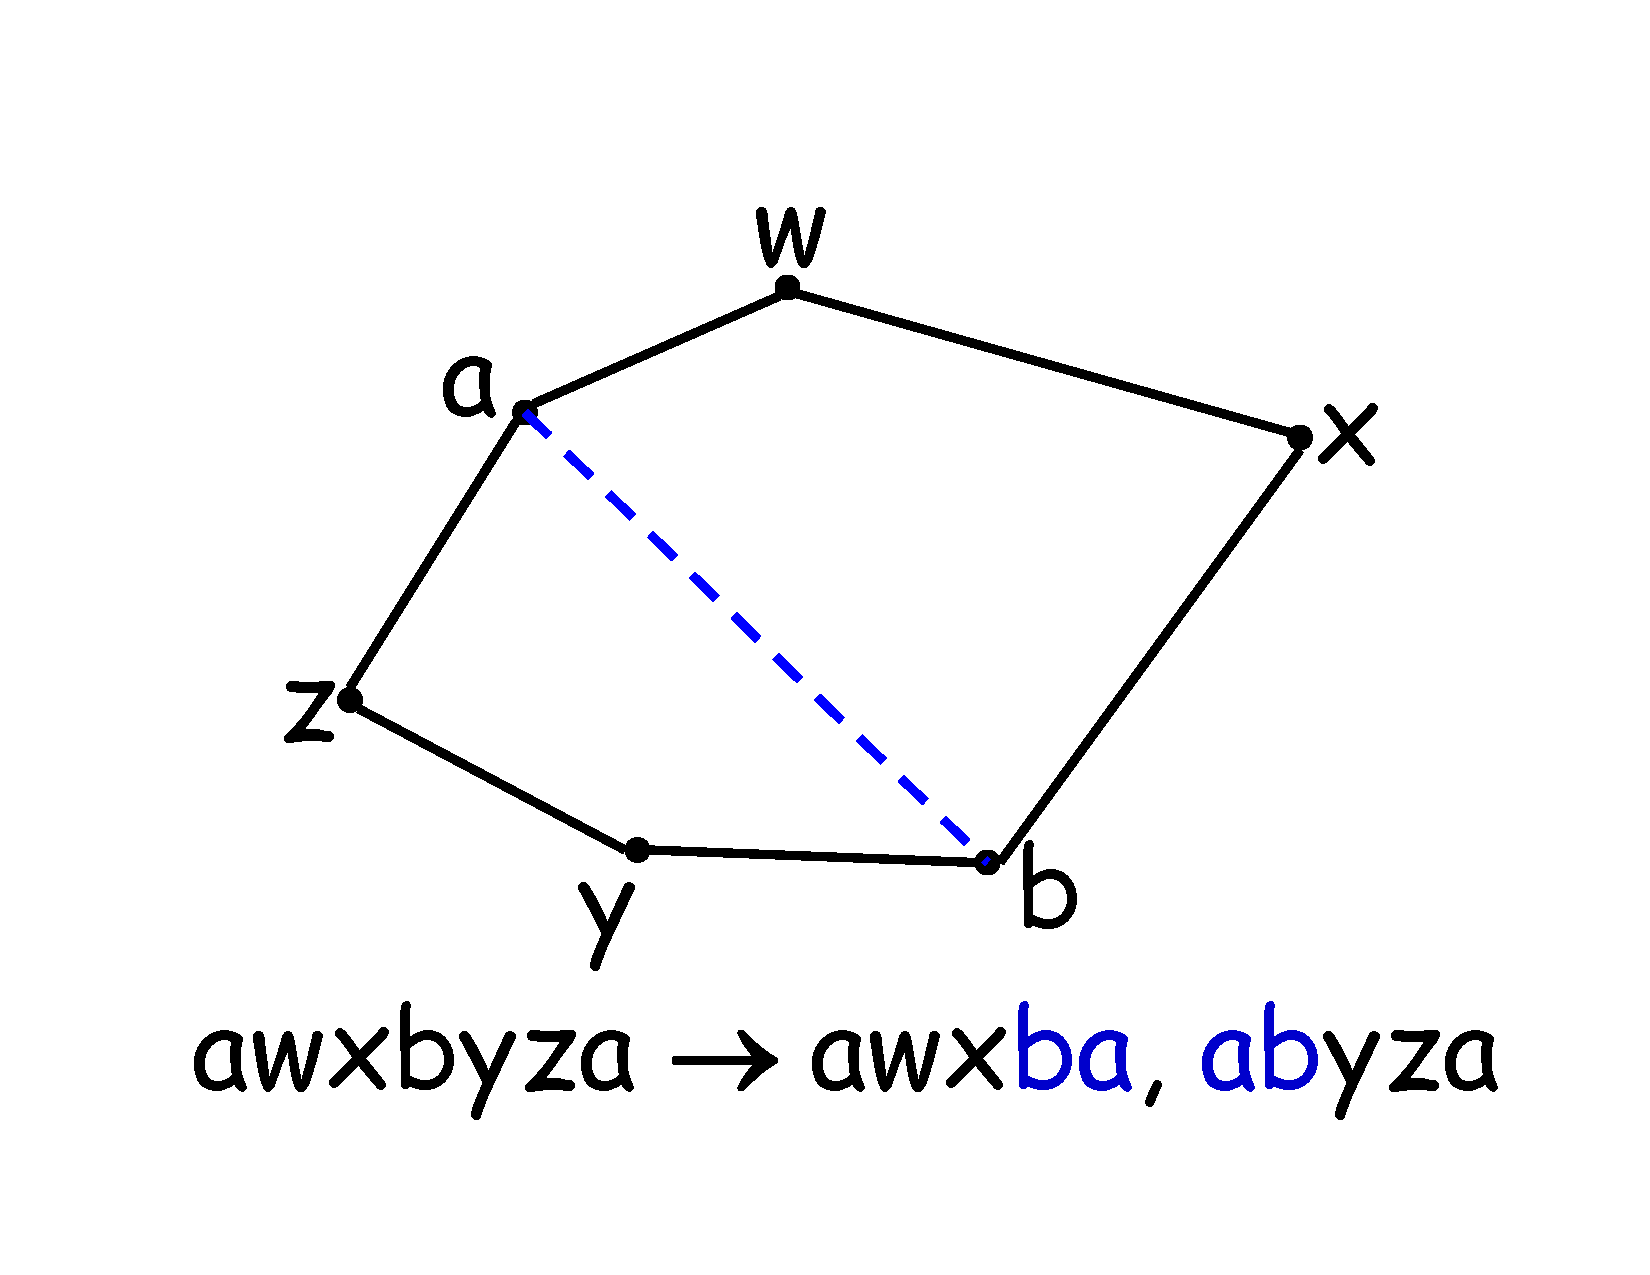
\includegraphics[height=2.5in]{figures/split-a-face}
%\caption{The Split a Face Case.}
%\label{fig:face-splitting}
%\end{figure}

\textbf{Constructor Case:} (add a bridge) Suppose $G$ and $H$ are
graphs with planar embeddings and disjoint sets of vertices.
Let $a$ be a vertex on a discrete face, $\gamma$, in the embedding of
$G$.  That is, $\gamma$ is of the form
\[
a\dots a.
\]
Similarly, let $b$ be a vertex on a discrete face, $\delta$, in the
embedding of $H$, so $\delta$ is of the form
\[
b\cdots b.
\]
Then the graph obtained by connecting $G$ and $H$ with a new edge,
$\edge{a}{b}$, has a planar embedding whose discrete faces are the union of
the discrete faces of $G$ and $H$, except that faces $\gamma$ and $\delta$
are replaced by one new face
\[
a\dots ab\cdots ba.
\]
%This is illustrated in Figure~\ref{fig:add-bridge}, where the faces of
%$G$ and $H$ are:
%\[
%G: \set{\texttt{axyza},\ \texttt{axya},\ \texttt{ayza}}
%    \qquad H: \set{\texttt{btuvwb},\ \texttt{btvwb},\ \texttt{tuvt}},
%\]
%and after adding the bridge $\edge{\texttt{a}}{\texttt{b}}$, there is a
%single connected graph with faces
%\[
%\set{\texttt{axyz{\color{blue}ab}tuvw{\color{blue}ba}},\
%         \texttt{axya},\ \texttt{ayza},\ \texttt{btvwb},\ \texttt{tuvt}}.
%\]
%\begin{figure}[h]
%\centering 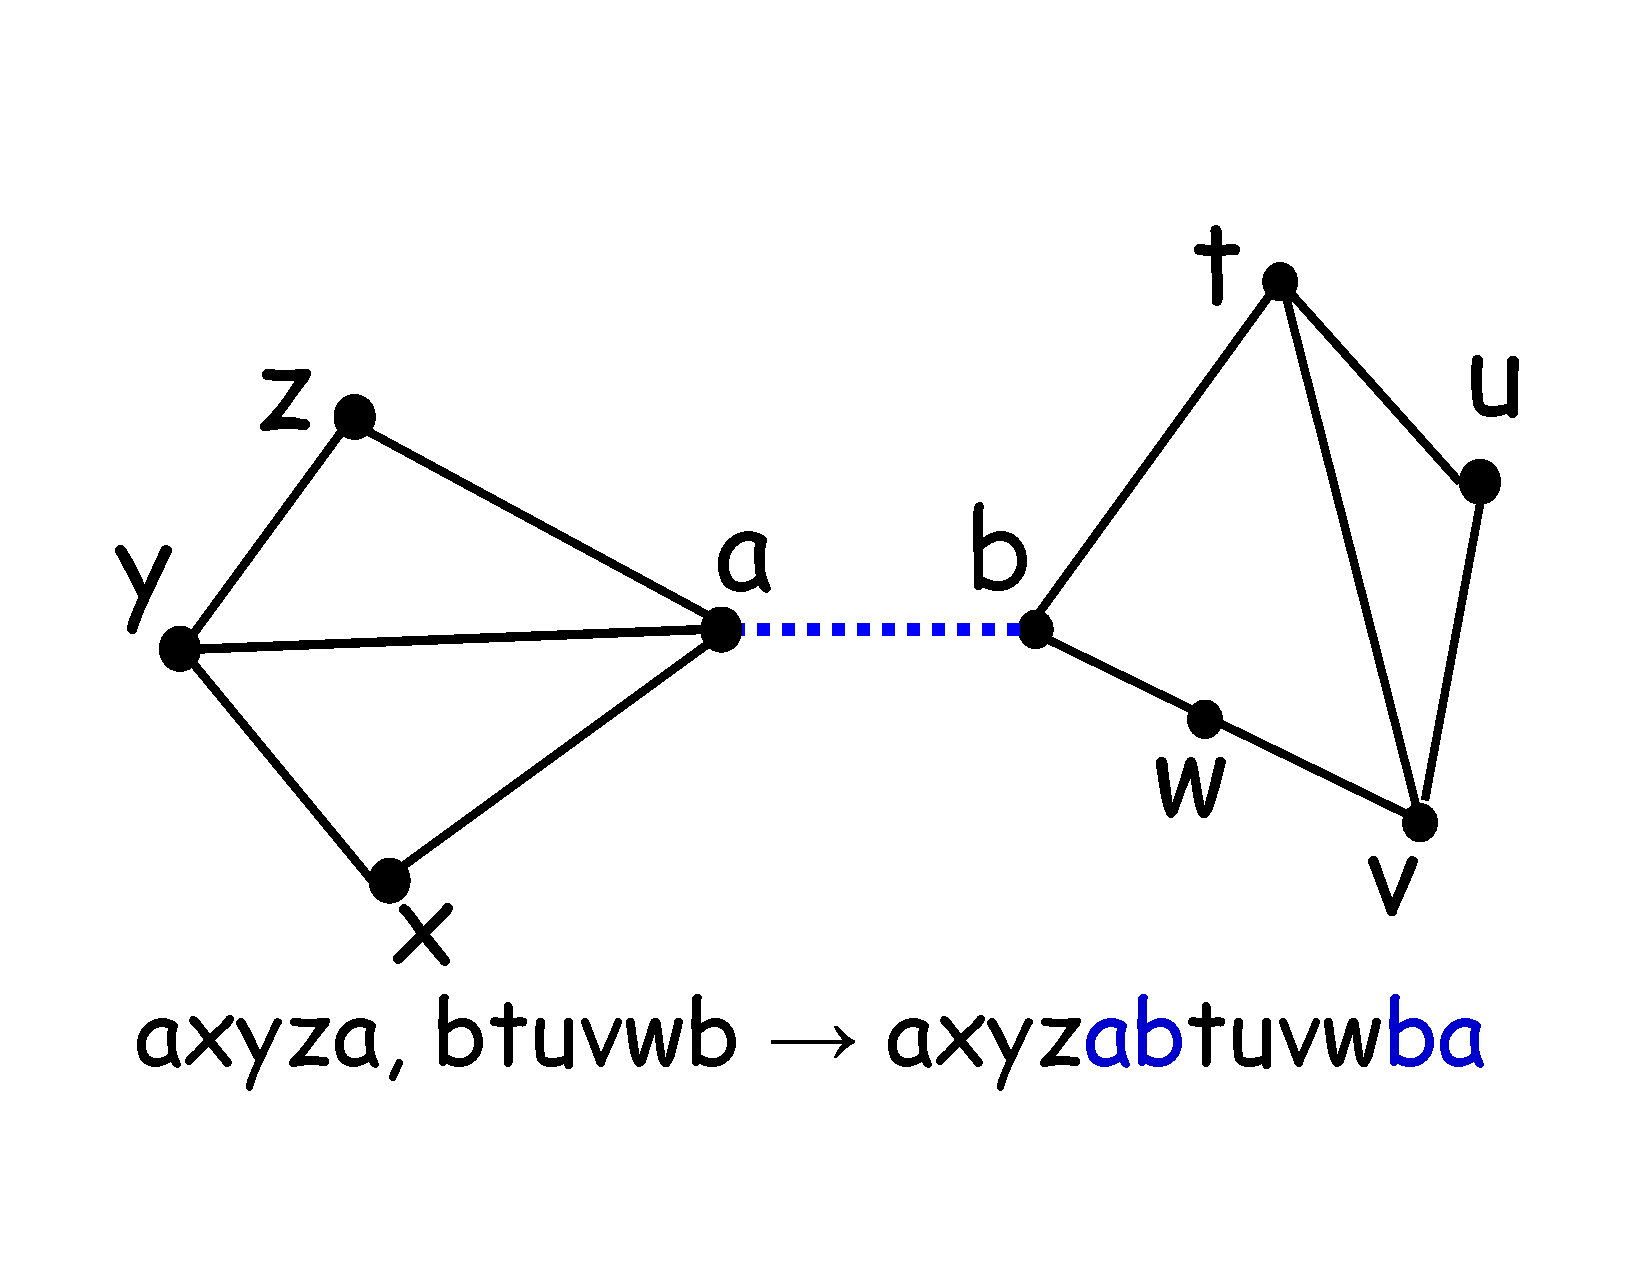
\includegraphics[height=3in]{figures/add-bridge}
%\caption{The Add Bridge Case.}
%\label{fig:add-bridge}
%\end{figure}

An arbitrary graph is \term{planar} iff each of it
has a planar embedding.

\end{definition*}
\end{minipage}}


\section{The Pulverizer}
Euclid's algorithm for finding the GCD of two numbers relies on
repeated application of the equation: 
\[
\gcd(a, b) = \gcd(b, \rem{a}{b})
\]
For example, we can compute the GCD of 259 and 70 as follows:
\[
\begin{array}{rclcl}
\gcd(259, 70)
    & = & \gcd(70, 49) & \quad & \text{since $\rem{259}{70} = 49$}\\
    & = & \gcd(49, 21) && \text{since $\rem{70}{49} = 21$} \\
    & = & \gcd(21, 7) && \text{since $\rem{49}{21} = 7$} \\
    & = & \gcd(7, 0) && \text{since $\rem{21}{7} = 0$} \\
    & = & 7.
\end{array}
\]
The Pulverizer goes through the same steps, but requires some extra
bookkeeping along the way: as we compute $\gcd(a, b)$, we keep track
of how to write each of the remainders (49, 21, and 7, in the example)
as a linear combination of $a$ and $b$ (this is worthwhile, because
our objective is to write the last nonzero remainder, which is the
GCD, as such a linear combination).  For our example, here is this
extra bookkeeping:
\[
\begin{array}{ccccrcl}
x & \quad & y & \quad & \rem{x}{y} & = & x - q \cdot y \\ \hline
259 && 70 && 49 & = &   259 - 3 \cdot 70 \\
70 && 49 && 21  & = &   70 - 1 \cdot 49 \\
&&&&            & = &   70 - 1 \cdot (259 - 3 \cdot 70) \\
&&&&            & = &   -1 \cdot 259 + 4 \cdot 70 \\
49 && 21 && 7   & = &   49 - 2 \cdot 21 \\
&&&&            & = &   (259 - 3 \cdot 70) -
                                2 \cdot (-1 \cdot 259 + 4 \cdot 70) \\
&&&&            & = &   \fbox{$3 \cdot 259 - 11 \cdot 70$} \\
21 && 7 && 0
\end{array}
\]

\section{RSA Encryption}
\begin{center}
\fbox{
\begin{minipage}[t]{6in}
\vspace{0.1cm}
\begin{description}

\item[Beforehand] The receiver creates a public key and a secret key
as follows.

\begin{enumerate}

\item Generate two distinct primes, $p$ and $q$.

\item Let $n = pq$.

\item Select an integer $e$ such that $\gcd(e, (p-1)(q-1)) = 1$.\\ The
{\em public key} is the pair $(e, n)$.  This should be distributed
widely.

\item Compute $d$ such that $de \equiv 1 \pmod{(p-1)(q-1)}$.\\ The
{\em secret key} is the pair $(d, n)$.  This should be kept hidden!

\end{enumerate}

\item[Encoding] The sender encrypts message $m$ to produce $m^\prime$ using
the public key:
\[
m' = \rem{m^e}{n}.
\]

\item[Decoding] The receiver decrypts message $m'$ back to message $m$
using the secret key:
\[
m = \rem{(m')^d}{n}.
\]

\end{description}

\vspace{0.1cm}
\end{minipage}
}
\end{center}

\section{Generating Functions}

Let $[x^n]F(x)$ denote the coefficient of $x^n$ in the power series
for $F(x)$.  Then,
\begin{equation}\label{1axk}
[x^n]\paren{\frac{1}{\paren{1-\alpha x}^k}} = \binom{n+k-1}{k-1}\alpha^n.
\end{equation}

\iffalse

\section{Convolution Counting}
Let
\begin{align*}
A(x) & = \sum_{n=0}^{\infty} a_n x^n, & B(x) & =
\sum_{n=0}^{\infty} b_n x^n, & C(x) & = A(x) \cdot B(x) =
\sum_{n=0}^{\infty} c_n x^n.
\end{align*}
Then
\[
c_n = a_0 b_n + a_1 b_{n-1} + a_2 b_{n-2} + \cdots + a_n b_0.
\]

\begin{mathrule*}[Convolution Rule]
  Let $A(x)$ be the generating function for selecting items from set
  $\mathcal{A}$, and let $B(x)$ be the generating function for selecting
  items from set $\mathcal{B}$.  If $\mathcal{A}$ and $\mathcal{B}$ are
  disjoint, then the generating function for selecting items from the
  union $\mathcal{A} \cup \mathcal{B}$ is the product $A(x) \cdot B(x)$.
\end{mathrule*}
\fi


\section{Finding a Generating Function}
The Fibonacci numbers are defined by:
\begin{align*}
f_0 & \eqdef 0 \\
f_1 & \eqdef 1 \\
f_n & \eqdef f_{n-1} + f_{n-2} \qquad \text{(for $n \geq 2$)}
\end{align*}

Let $F$ be the generating function for the Fibonacci numbers,
that is,
\[
F(x) \eqdef f_0 + f_1 x + f_2 x^2 + f_3 x^3 + f_4 x^4 + \cdots
\]
So we need to derive a generating function whose series has
coefficients:
\[
\ang{0,\ 1,\ f_1 + f_0,\ f_2 + f_1,\ f_3 + f_2,\ \dots}
\]
Now we observe that
\[
\begin{array}{ccccccccccl}
  & \langle & 0, & 1, & 0, & 0, & 0, & \dots & \rangle
    &     & x \\
+ & \langle & 0, & f_0, & f_1, & f_2, & f_3, & \dots & \rangle
    &     & x F(x) \\
+ & \langle & 0, & 0, & f_0, & f_1, & f_2, & \dots & \rangle
    &     & x^2 F(x) \\ \hline
  & \langle & 0, & 1 + f_0, & f_1 + f_0, & f_2 + f_1, & f_3 + f_2, & \dots & \rangle
    &     & x + x F(x) + x^2 F(x) \\
\end{array}
\]
%
This sequence is almost identical to the right sides of the
Fibonacci equations.  The one blemish is that the second term is
$1 + f_0$ instead of simply 1.  But since $f_0 = 0$, the second
term is ok.

So we have
\begin{align}
F(x) & = x + x F(x) + x^2 F(x). \notag\\
F(x) & = \frac{x}{1 - x - x^2}.\label{Fx}
\end{align}

\section{Partial Fractions}

Here's a particular case of the Partial Fraction Rule that should be
enough to illustrate the general Rule.  Let
\[
r(x) \eqdef \frac{p(x)}{(1-\alpha x)^2 (1-\beta x) (1-\gamma x)^3}
\]
where $\alpha, \beta, \gamma$ are distinct complex numbers, and $p(x)$ is
a polynomial of degree less than the demoninator, namely, less than 6.
Then there are unique numbers $a_1,a_2,b,c_1,c_2,c_3 \in \complexes$ such
that
\[
r(x)
= \frac{a_1}{1-\alpha x} + \frac{a_2}{(1-\alpha x)^2}
+ \frac{b}{1-\beta x}
+ \frac{c_1}{1-\gamma x} + \frac{c_2}{(1-\gamma x)^2} + \frac{c_3}{(1-\gamma x)^3}
\]


%%%%%%%%%%%%%%%%%%%%%%%%%%%%%%%%%%%%%%%%%%%%%%%%%%%%%%%%%%%%%%%%%%%%% 
% Appendix ends here 
%%%%%%%%%%%%%%%%%%%%%%%%%%%%%%%%%%%%%%%%%%%%%%%%%%%%%%%%%%%%%%%%%%%%% 

\end{document}
